\section{Sprachmodelle}

    \subsection{Überblick}
    \label{sec:langmodels}
    	In diesem Abschnitt sollen die theoretischen Aspekte der Wortvorhersage erleutert werden. Es handelt sich hier um das Themengebiet des \emph{Natural Language Processing}. In diesem Abschnitt werden dazu ausschließlich Sprachmodelle behandelt. Um Annahmen darüber zu machen, welche Wörter nach einem anderen folgen können, benötigt man zunächst einmal ein Modell der verwendeten Sprache. Im optimalen Fall kann ein \emph{Sprachmodell} eine Sprache und die Beziehung zwischen Wörtern umfassend abbilden. In \autoref{sec:design-learnerPredictor} wird ein \emph{Sprachmodell} als Sammlung von Dateien mit Informationen über einen Text definiert. In diesem Abschnitt geht es um die Bedeutung dieser Informationen.
        
        Eine naheliegende Möglichkeit ein Modell einer Sprache zu generieren ist das Formulieren einer \emph{Grammatik}. Hierbei wird versucht die sytaktischen Regeln einer Sprache zu definieren. Im entworfenen Prototypen spielen solche \emph{Grammatiken} keine Rolle. Darum werden diese nur sehr kurz erklärt.
        
        Ein Beispiel einer einfachen Grammatik ist in \autoref{fig:grammer} zu sehen. \texttt{S -> NP VP} beschreibt, dass ein Satz \texttt{S} aus einem \emph{Noun Phrase} \texttt{NP} und einem \emph{Verb Phrase} \texttt{VP} bestehen kann. Alle weiteren Regeln funktionieren entsprechend. Mit Hilfe einer solchen Grammatik ist es möglich die Funktion eines Wortes innerhalb von einem Satz zu bestimmen. Dieser kann dann, wie in \autoref{fig:parsingTree} zu sehen,  als \emph{tree} dargestellt werden. Im Beispiel gilt es zu beachten, dass \autoref{fig:grammer} nicht alle in \autoref{fig:parsingTree} enthaltenden Worte enthält und somit erst einmal nicht funktionieren würde.
        
        Folgen wir also folgender vereinfachten Regel: Innerhalb eines \emph{Preposition Prase} \texttt{PP} nach einer Preposition \texttt{P} und einem Determinator \texttt{DET} muss immer ein Nomen \texttt{N} kommen. Dann können wir in dem Satzteil \texttt{in the …} aus \autoref{fig:parsingTree} nur noch Nomen als Folgewort vorschlagen.
        
        \begin{figure}[H]
			\centering
            \begin{subfigure}{0.49\textwidth}
				\begin{lstlisting}
S -> NP VP
VP -> V NP | V NP PP
PP -> P NP
V -> "saw" | "ate" | "walked"
NP -> "John" | "Mary" | "Bob" | Det N | Det N PP
Det -> "a" | "an" | "the" | "my"
N -> "man" | "dog" | "cat" | "telescope" | "park"
P -> "in" | "on" | "by" | "with"
    			\end{lstlisting}
                \caption{Einfache Grammatik}
                \label{fig:grammer}
			\end{subfigure}
            \begin{subfigure}{0.49\textwidth}
            	\centering
            	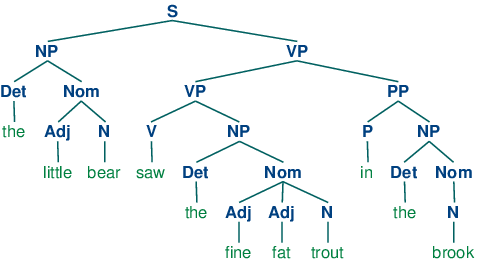
\includegraphics[width=.8\linewidth]{images/grammer.png}
            	\caption{\emph{parsing tree}}
            	\label{fig:parsingTree}
            \end{subfigure}
            \label{fig:grammerWithTree}
            \caption{Beispiel einer einfachen \emph{Grammatik} \parencite[Kapitel 8]{nltk:book}}
        \end{figure}
        \newpage
        
        Allerdings stößt man, wie von \cite[S. 544]{jamia:introduction} im Abschnitt \emph{The limitations of hand-written rules: the rise of statistical NLP} aufgefürht wird, mit solchen \emph{Grammatiken} an Grenzen. In dem Artikel werden zwei Probleme solcher \emph{Grammatiken} beschrieben.
    
    	Zum einen beschreiben diese in erster Linie Syntax und nicht die Semantik eines Satzes. Dies kann laut \cite{jamia:introduction} zwar durch Erweitern der Regeln gelöst werden. Sie Nutzen hier das Beispiel, dass das Verb \texttt{essen} nur für bestimmte \emph{essbare} Nomen gültig gemacht werden kann. Weißen aber darauf hin, dass so die Regeln viel zu komplex und unüberschaubar würden.
        
        Als zweites Problem führen sie an das solche \emph{Grammatiken} mit Sätzen, die zwar von Menschen verstanden werden aber nicht unbedingt grammatischen Regeln folgen, nicht umgehen können.
        
        \cite{jamia:introduction} beziehen sich bei Ihren Überlegungen, auch wenn sie Anwendungsbeispiele aus der Medizin nutzen, auf \emph{Natural Language Processing} im Allgemeinen. Hier soll versucht werden diese Formulierungen bezüglich der Wortvorhersage zu verwenden.
        
        Aufgrund der genannten Probleme gab es, wie \cite{jamia:introduction} auf Seite 545 schließen, in den 1980ern eine Wende hin zu \emph{statistischem Natural Languge Processing}. Sie erklären \enquote{[\dots]fewer, broader rules replace numerous detailed rules, with statistical-frequency information looked up to disambiguate.} Übersetzt meinen sie also, dass weniger aber weiter gefasste Regeln in Kombination mit statistischen Frequenzen detaillierte Regeln ersetzen. Ein Beispiel für solche statistische Modelle sind die in \autoref{sec:n-gramms} erklärten \emph{N-gramms}.
        
        Ein statistisches Modell basiert immer auf Wahrscheinlichkeiten. Im gleichen Abschnitt beschreiben \cite{jamia:introduction} auch, dass diese Wahrscheinlichkeiten abhängig sind von dem Text aus welchem die Statistiken generiert werden. So liefert vereinfacht Formuliert eine auf Prosa Texten gelernte Statistik keine guten Ergebnisse auf Wissenschaftliche Texte.  
        
    \newpage
    \subsection{N-gramms}
    \label{sec:n-gramms}
    
    	Um Informationen über ein Wort in einem Text zu erhalten ist eine Möglichkeit sich die Umgebung dieses Wortes anzusehen. Ein \emph{N-gramm} besteht also aus einem Wort und den \emph{N-1} vorherigen Wörtern an einer Textstelle. Mit diesen Informationen können wir auch eine Sprache so beschreiben, dass wir Wortvrhersagen machen können. \parencite[S. 468, Gleichung 1]{cumpatationalLinguistics:classBasedNGramms} machen dazu die in \autoref{eq:wordChain} gezeigte Annahme.
        
        \begin{equation}
        	Pr(w_1^k) = Pr(w_1) Pr(w_2|w_1) \cdots Pr(w_k|w_1^{k-1})
        	\label{eq:wordChain}
        \end{equation}
        
        Sie betrachten also die Wahrscheinlichkeit eines Wortes abhängig von seinen Vorgängern \(Pr(w_k|w_1^{k-1})\). Und definieren die Wahrscheinlichkeit einer Wortkette \(Pr(w_1^k)\) als Summe dieser Wahrscheinlichkeiten. In dem online Buch \parencite{nlwp:book} wird dazu unter Abschnitt 3.8 eine gute Erklärung geliefert. Zunächst formulieren de Kok und Brouwer die Formel neu mit einem Beispielsatz. Hier wird dazu in \autoref{eq:wordChainWithWords} der Satz \texttt{ich war gestern abend essen} verwendet werden.
        
        \begin{equation}
        	\begin{split}
        		Pr(\text{ich war gestern abend essen}) \\
                = Pr(\text{ich}) Pr(\text{war}|\text{ich}) Pr(\text{gestern}|\text{ich war}) \\
                Pr(\text{abend}|\text{ich war gestern}) Pr(\text{essen}|\text{ich war gestern abend}) 
            \end{split}
            \label{eq:wordChainWithWords}
        \end{equation}
        
        Im gleichen Abschnitt erklären sie, dass ein \emph{korrekter} Satz eine höhere Wahrscheinlichkeit haben wird als ein fehlerhafter. Interessant ist hier was als \emph{korrekt} verstanden wird. Da sich diese Wahrscheinlichkeiten auf aus Trainingstexten gelernten Statistiken beziehen. So kann ein viel verwendeter grammatisch unkorrekter Satz auch eine hohe Wahrscheinlichkeit haben. Das ist eine durchaus erwünschte Eigenschaft solcher Modelle.
        
        In \parencite{nltk:book} unter Abschnitt 1.1 von Kapitel 8 wird sehr schön gezeigt, dass es theoretisch unendlich solcher \emph{korrekter} Sätze gibt. Es ist also unmöglich, selbst mit sehr großen Trainingstexten eine Sprache komplett abzubilden und mit \autoref{eq:wordChain} für jeden denkbaren Satz Wahrscheinlichkeiten zu berechnen. 
        
        De Kok und Brouwer erwähnen auch, dass es sich bei \autoref{eq:wordChain} um eine Markow-Kette handelt. Sie fahren fort, dass wir auf die Kette nun auch die Markow-Annahme anwenden können. Diese formulieren sie übersetzt als: \enquote{Die Vorhersage des nächsten Zustands ist nur Abhängig von dem aktuellen Zustand.}\parencite[Abs.  3.8]{nlwp:book}
        
        \autoref{eq:markov-assumtion} zeigt \parencite[Abs.  3.8, Gleichung 3.8]{nlwp:book} in leicht veränderter Schreibweise um innerhalb dieser Arbeit konsitente Bezeichnungen zu verwenden.  
        
        \begin{equation}
        	Pr(w_k|w_1^{k-1}) \approx Pr(w_k|w_{k-1})
        	\label{eq:markov-assumtion}
        \end{equation}
        
        Dieses vereinfachte Modell nennt sich \emph{bigramm} Modell. Die Übergangswahrscheinlickeit von \(w_{k-1}\) nach \(w_k\) lässt sich einfach mit \autoref{eq:bigramm-prob} berechnen. Dabei handelt es sich um \parencite[Abs.  3.8, Gleichung 3.9]{nlwp:book} wieder mit angepasster Schreibweise.
        
        \begin{equation}
        	Pr(w_k|w_{k-1}) = \frac{C(w_{k-1};w_k)}{C(w_{k-1})}
        	\label{eq:bigramm-prob}
        \end{equation}
    	
    	\(C(w_{k-1};w_k)\) gibt an wie oft im Trainingstext das Wort \(w_{k-1}\) direkt vor \(w_k\) steht. \(C(w_{k-1})\) ist die Häufigkeit des Wortes \(w_{k-1}\) im Trainingstext. Zum besseren Verständniss wird dies in \autoref{eq:bogramm-prob-words} noch einmal mit Beispielworten dargestellt.
        
        \begin{equation}
        	Pr(\text{war}|\text{ich}) = \frac{C(\text{ich};\text{war})}{C(\text{ich})}
        	\label{eq:bogramm-prob-words}
        \end{equation}
        
        
        Es ist möglich die Qualität der Vorhersage zu verbessern, wenn man nun nicht nur das vorherige Wort sondern die zwei vorherigen Worte betrachtet. Oder auch, sich \autoref{eq:wordChain} wieder annähernd, die \(N - 1\) vorherigen Worte. Umso größer \emph{N} jedoch wird desto unwahrscheinlicher wird es, dass ein \emph{N-gramm} auch im Trainingstext vorkommt. So werden die Kombinationen \texttt{ich bin} und \texttt{ich war} in einem ausreichend großem Text oft genug vorkommen um gute Aussagen über ihre Wahrscheinlichkeit machen zu können. Bei einer Kombination \texttt{ich war gestern abend} ist schon ein einmaliges Vorkommen nicht unbedingt gegeben.
        
        Da diese Wahrscheinlichkeiten mit Hilfe eines Trainingstextes angelernt werden, besteht die Gefahr, dass das Modell zu stark auf die Trainingsdaten abgestimmt ist. Kommt beispielsweise das Wort \texttt{Armatur} nicht in den Trainigsdaten vor, kann man bei ausreicheichend langen Trainingstexten davon ausgehen, dass es sich dabei um ein seltenes Wort hadelt. Dennoch würde in diesem Fall dem Wort nicht nur eine kleine Wahrscheinlichkeit, sondern eine Wahrscheinlichkeit von 0 zugeteilt. Dies gilt nicht nur für alleinstehende Worte sondern auch für seltene Wortkombinationen. Dieses Problem nennt sich \emph{data sparsity} und wird unter anderem auch in einem von Studenten der TU-München erstellten Wiki von \parencite[Abs. 5]{recognize-speech:n-gramms} beschreiben. 
        
        Das Abschwächen dieses Effektes nennt sich \emph{smoothing}. Der einfachste \emph{smoothing} Ansatz für \emph{N-gramm} Modelle ist der \emph{Backoff Approach}. Auch dieser wird im oben erwähnten Wiki in \parencite{recognize-speech:backoff} erklärt. Dabei wird sobald ein gesuchtes \emph{N-gramm} nicht gefunden wird einfach auf das nächst kürzere Modell zurückgegriffen. Ist die Wahrscheinlichkeit \(Pr(\text{gestern}|\text{ich war}) = 0\) versucht man eine Vorhersage anhand von \(Pr(\text{gestern}|\text{war})\) zu treffen. Das auch von Pfeuffer erläuterte Problem hierbei ist, dass man nun Wahrscheinlichkeiten aus zwei verschiedenen Modellen miteinander mischt. Darum werden von ihm noch weitere \emph{smoothing} Ansätze vorgestellt die beide Modelle inneinader verrechnen. Auf diese wird hier nicht weiter eingegangen, da sie für den entwickelten Prototypen keine Rolle spielen.
        
    \newpage
	\subsection{Klassenbasierte n-gramm Sprachmodelle}
    \label{sec:brownClustering}
    
    	-> exmple from brown: next Monday != next Thuesday
        -> is some kind of smoothing
        -> rertive cluster by assumtion:
    
    	\begin{equation}
   			P(w_i|w_{i-1}) = P(w_i|c_i) P(c_i|c_{i-1})
        	\label{eq:wordPropability}
		\end{equation}
        
        -> explain buttom up algorythm
        
    \newpage    
    \subsection{Corpora}
    	Die für \emph{Statistische Sprachmodelle} verwendeten Trainingstexte werden auch als \emph{Textcorpus} bezeichnet. Wie bereits in \autoref{sec:langmodels} erwähnt kann eine Thematische ausrichtung des Corpus ein Sprachmodell stark beinflussen. So können aus unterschiedlichen Themenfeldern bezogene Texte nicht nur unterschiedliche Häufigkeiten, sondern auch ein unterschiedliches Vokabular haben.
        
        Es kann nun also versucht werden einen \emph{Corpus} zu bilden der eine Sprache möglichst umfassend und in möglichst vielen Themenbereichen abbildet. Die Penn Treebank wäre ein Beispiel für einen solchen \emph{Corpus} für die Englische Sprache. Ein anderer Ansatz wäre das Sprachmodell auf ein bestimmtes Themengebiet zu speialisieren (wie claßen paper mit medizin????). Es ist zu erwarten, dass ein solches Modell zwar im Allgemeinen schlechtere Vorhersagen treffen kann, dafür aber in seinem Themengebiet besser als ein allgemeines Modell abschneidet.
        
        Um dem in \autoref{sec:n-gramms} erwähnten Problem der \emph{data sparsity} vorzubeugen muss ein \emph{Corpus} ausreichend groß sein. Brown u. a. nutzen für ihre versuche \emph{Corpusgrößen} von xxx xxx und sogar xxx (cite). Die Penn Treebank umfasst xxxx Worte (cite). Umso kleiner ein Corpus ist, desto stärker wird er nur den gelernten Text beschreiben und nicht eine Sprache im allgemeinen.
    \newpage
    
